%%%%%%%%%%%%%%%%%%%%%%%%%%%%%%%%%%%%%%%%%
% Journal Article
% LaTeX Template
% Version 1.3 (9/9/13)
%
% This template has been downloaded from:
% http://www.LaTeXTemplates.com
%
% Original author:
% Frits Wenneker (http://www.howtotex.com)
%
% License:
% CC BY-NC-SA 3.0 (http://creativecommons.org/licenses/by-nc-sa/3.0/)
%
%%%%%%%%%%%%%%%%%%%%%%%%%%%%%%%%%%%%%%%%%

%----------------------------------------------------------------------------------------
%	PACKAGES AND OTHER DOCUMENT CONFIGURATIONS
%----------------------------------------------------------------------------------------

\documentclass{article}

%\documentclass{aastex}  % version 5.0 or prior
%\usepackage{natbib}

\usepackage[table,x11names]{xcolor}
\usepackage{array}
\usepackage{graphicx}
\usepackage{lipsum} % Package to generate dummy text throughout this template
%\usepackage[sc]{mathpazo} % Use the Palatino font
\usepackage[T1]{fontenc} % Use 8-bit encoding that has 256 glyphs
\linespread{1.05} % Line spacing - Palatino needs more space between lines
\usepackage{microtype} % Slightly tweak font spacing for aesthetics

\usepackage[margin=1in,columnsep=20pt]{geometry} % Document margins
\usepackage{multicol} % Used for the two-column layout of the document
\usepackage[hang, small,labelfont=bf,up,textfont=it,up]{caption} % Custom captions under/above floats in tables or figures
\usepackage{booktabs} % Horizontal rules in tables
\usepackage{float} % Required for tables and figures in the multi-column environment - they need to be placed in specific locations with the [H] (e.g. \begin{table}[H])
\usepackage{hyperref} % For hyperlinks in the PDF
\usepackage{subcaption}

\usepackage{lettrine} % The lettrine is the first enlarged letter at the beginning of the text
\usepackage{paralist} % Used for the compactitem environment which makes bullet points with less space between them
\usepackage{amsmath}
\usepackage{abstract} % Allows abstract customization
\renewcommand{\abstractnamefont}{\normalfont\bfseries} % Set the "Abstract" text to bold
\renewcommand{\abstracttextfont}{\normalfont\small\itshape} % Set the abstract itself to small italic text

\usepackage{titlesec} % Allows customization of titles
%\renewcommand\thesection{\Roman{section}} % Roman numerals for the sections
%\renewcommand\thesubsection{\Roman{subsection}} % Roman numerals for subsections
%\renewcommand\thesubsubsection{\Alph{subsubsection}} % Roman numerals for subsections
\titleformat{\section}[block]{\Large\scshape}{\thesection}{1em}{} % Change the look of the section titles
\titleformat{\subsection}[block]{\large}{\thesubsection}{1em}{} % Change the look of the section titles
\titleformat{\subsubsection}[block]{}{\thesubsubsection}{1em}{} % Change the look of the section titles

\usepackage{fancyhdr} % Headers and footers
\pagestyle{fancy} % All pages have headers and footers
\fancyhead{} % Blank out the default header
\fancyfoot{} % Blank out the default footer
\fancyhead[C]{Montana State University \quad $\bullet$ \quad CSCI 466 Artificial Intelligence \quad $\bullet$ \quad Group 21} % Custom header text
\fancyfoot[RO,LE]{\thepage} % Custom footer text

\newcommand{\ve}[1]{\boldsymbol{\mathbf{#1}}}

%----------------------------------------------------------------------------------------
%	TITLE SECTION
%----------------------------------------------------------------------------------------

\title{\vspace{-15mm}\fontsize{24pt}{10pt}\selectfont\textbf{CSCI 446 Artificial Intelligence \\ Project 2 Final Report} \\[-2mm]} % Article title
\date{\today}
\author{
\large
\textsc{Roy Smart} \and \textsc{Nevin Leh} \and \textsc{Brian Marsh}\\[2mm] % Your name
}


%----------------------------------------------------------------------------------------

\begin{document}

\maketitle % Insert title

\thispagestyle{fancy} % All pages have headers and footers

%\begin{abstract}
%We present a novel way of performing MOSES data inversions using a
%\end{abstract}

%----------------------------------------------------------------------------------------
%	ARTICLE CONTENTS
%----------------------------------------------------------------------------------------

%\begin{multicols}{2} % Two-column layout throughout the main article text
\normalsize

\begin{abstract}

	Our project attempts to solve the classification problem of machine learning using four different algorithms.  
	Each algorithm is tested on five datasets which train it to obtain enough knowledge to make an educated classification of new data points.  
	After training, the algorithms were tested to classify a new data point, then measured on their precision and convergence for correct answers.  
	The precision scores of the algorithms were comparable across all the datasets, with a clear leader being difficult to distinguish in any of the datasets.
	
\end{abstract}
\section{Introduction}

	In a broad sense, machine learning refers to efforts to giving computers the ability to learn without explicit instructions. 
	Machine learning algorithms (MLAs) have been shown to be successful at solving a wide range of problems.  
	One common problem in this realm of machine learning is known as classification. 
	Classification is a problem that can be solved using several algorithms, but the effectiveness of the algorithm depends greatly upon the specific dataset involved.
	  
	We implemented four machine learning algorithms (MLAs) to attempt to classify new data points into sets based upon previous information gained through training.  
	The algorithms used are $k$-Nearest Neighbors, Naive Bayes, Tree Augmented Naive Bayes (TAN), and Iterative Dichotomiser 3 (ID3).  
	Additionally, each algorithm is tested with five different datasets: the Wisconsin Breast Cancer Database, the Glass Identification Database, the Iris Plants Database, the Small Soybean Database, and the 1984 United States Congressional Voting Records Database.  
	The effectiveness of each algorithm is measured by the metrics of precision and convergence.  

\section{Datasets}

	In this project we are asked to train our MLAs on five different datasets, each with a different set of challenges to our MLAs. 
	For example, the soybean dataset is really small, the cancer database is reasonably large, and the attributes in the glass dataset are not very well correlated (as we will soon see).
	
	A problem with some of the datasets is that the contain ID numbers, numbers that are different for every member in the dataset. These are problematic for our algorithms as the ID number does not provide any useful information, and it hurts the predictive power of our algorithms. Therefore we have edited out all ID numbers from the datasets under the assumption that any researcher attempting to solve real-world machine learning problems would also ignore the ID numbers.
	
	\subsection{Discretization}
	
		Two datasets, the iris dataset and the glass dataset have continuous values. 
		We are asked to discretize these dataset to more accurately compare the different MLAs.
		For our project, we adopted \textit{binning} as our discretization scheme.
		Binning is a simple method for discretization that defines a certain number of adjacent intervals, known as bins, and then replaces points that fall within each bin by a value representative of that bin.
		
		For the data in this report the number of bins was set to 10. In principle, the ideal number of bins in terms of MLA precision could be any integer larger than one, but through tests we found that the ideal number of bins is proportional to the number of classes in the dataset.
	
	\subsection{Cross-Validation}
	
		Cross-validation is statistical bootstrapping techinque used to estimate the generality of a statistical model using a dataset independent of the dataset used to create the model. 
		In the context of machine learning, this means that we will partition the full datasets into training and validation datasets. 
		For this project we are asked to use the so-called $k$-fold cross validation technique, where the full dataset is partitioned into training and testing datasets through the use of \textit{folds}. 
		The folds are found by splitting the dataset into $k$ equal sized pieces, and assigning each piece to be a fold. 
		One fold is selected as the validation set, and the rest of the folds are assigned to the training set. 
		This process is then repeated $k$ times, where each fold is taken to be the validation set once.
	
		To further increase the accuracy of our cross-validation process, we will \textit{stratify} the folds described by $k$-fold cross-validation technique. 
		Stratification in this context means that each fold will have an equal distribution of the classes in each dataset..
		This process makes cross-validation more accurate, because it gives each MLA adequate information on each class for every training dataset.
		Without stratification, some training datasets could give a MLA zero examples of a particular class, hurting the MLA's ability to generalize.
		
		In $k$-fold cross-validation, $k$ is a free parameter that can be tuned by the user. For this project, we have selected $k = 10$, because it will allow us to perform the convergence tests discussed in Section \ref{conv} over a larger range.
	
	\subsection{Missing Values}
	
		Some of the datasets have missing values. 
		This is problematic since most of the MLAs will yield vastly different answers if some data is missing. 
		However, we note that the appearance of missing values in the voting dataset is merely an illusion, missing values in this dataset can signify a stance on a particular issue and this information should be used by our algorithms. 
		
		Since we have determined that the voting set contains no missing values, the only remaining dataset with missing values is the cancer dataset. Since there are so few missing values and the dataset is so large, we have decided to simply delete any data with missing values from the cancer dataset. Therefore, we have found that data imputation is not necessary for this project. 
	
\section{$k$-Nearest Neighbors}
	\subsection{Training}
		K-Nearest Neighbors attempts to solve the classification problem by using already-known data points with similar characteristics to make an educated guess of the class.  The training for k-Nearest Neighbors involves simply reading in all of the dataset and storing these records as points based on their values.
		\subsubsection{Constructing Probability Table}
	\subsection{Validation}
		\subsubsection{Value Distance Metric}
			The classification in k-Nearest Neighbors is found using the classes of the neighboring data points.  These neighboring points are found by calculating the distances to each point in the training set to the new point using the Minkowski distance metric.  This metric includes a value p that can be changed to tune the effectiveness of the algorithm.  The neighbors used in classification are those data points with the smallest Minkowski distance.
		\subsubsection{Determining $k$ and $p$}
			The effectiveness of the k-Nearest Neighbors algorithm depends heavily on the values used for the number of neighbors (k) and the power used in the distance equation (p).  Our test used varying values of k between 1 and 20 and of p between 1 and 9.  While the precision of the algorithm with regards to the values of k and p was highly variable for different datasets, overall, higher precision was generally found with higher values of p.  The value of p had a lesser effect, with very low values seemingly being favorable.
			\begin{figure}[h!]
				\centering
				\begin{subfigure}[b]{0.32\textwidth}
					\centering
					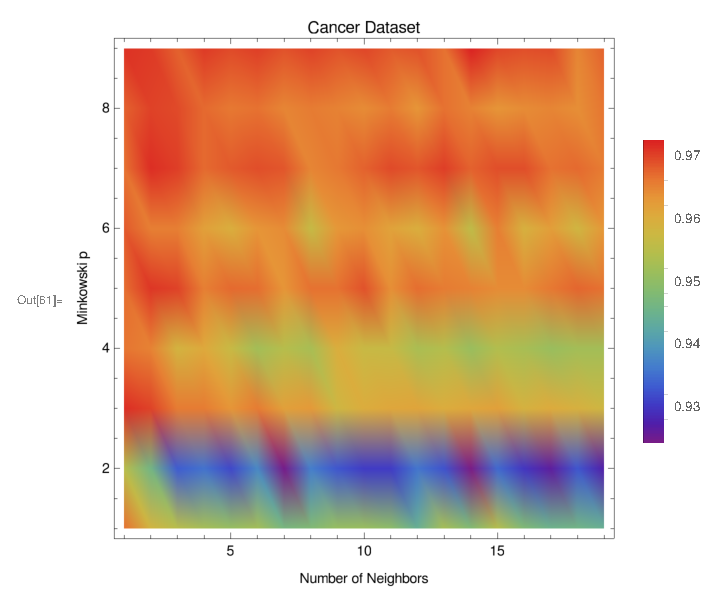
\includegraphics[width=\textwidth]{figs/kNN/cancer_plot_kp}	
					\caption{}
					\label{kp_cancer}				
				\end{subfigure}	\	
				\begin{subfigure}[b]{0.32\textwidth}
					\centering
					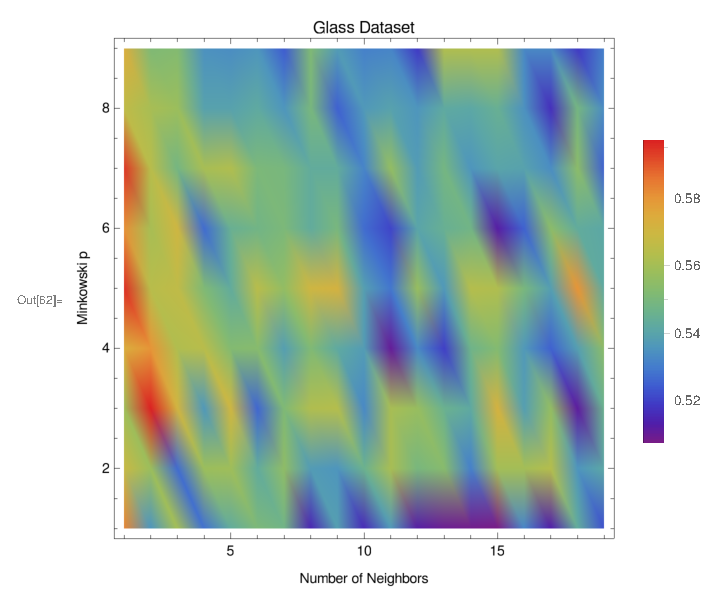
\includegraphics[width=\textwidth]{figs/kNN/glass_plot_kp}
					\caption{}
					\label{kp_glass}					
				\end{subfigure} \	
				\begin{subfigure}[b]{0.32\textwidth}
					\centering
					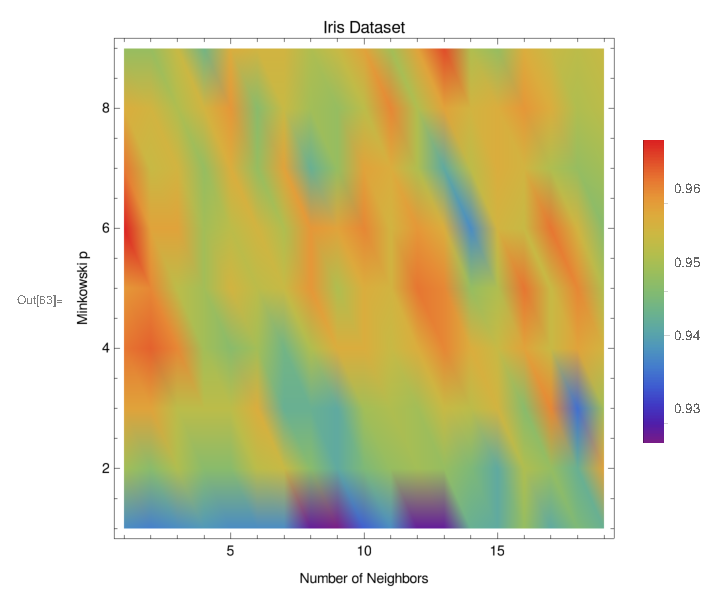
\includegraphics[width=\textwidth]{figs/kNN/iris_plot_kp}	
					\caption{}
					\label{kp_iris}				
				\end{subfigure} \	
				\begin{subfigure}[b]{0.32\textwidth}
					\centering
					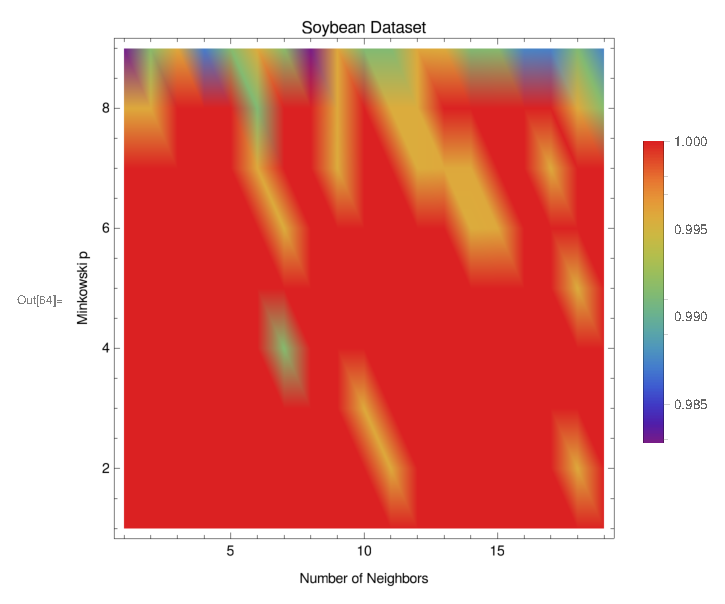
\includegraphics[width=\textwidth]{figs/kNN/soybean_plot_kp}	
					\caption{}
					\label{kp_soybean}				
				\end{subfigure} \	
				\begin{subfigure}[b]{0.32\textwidth}
					\centering
					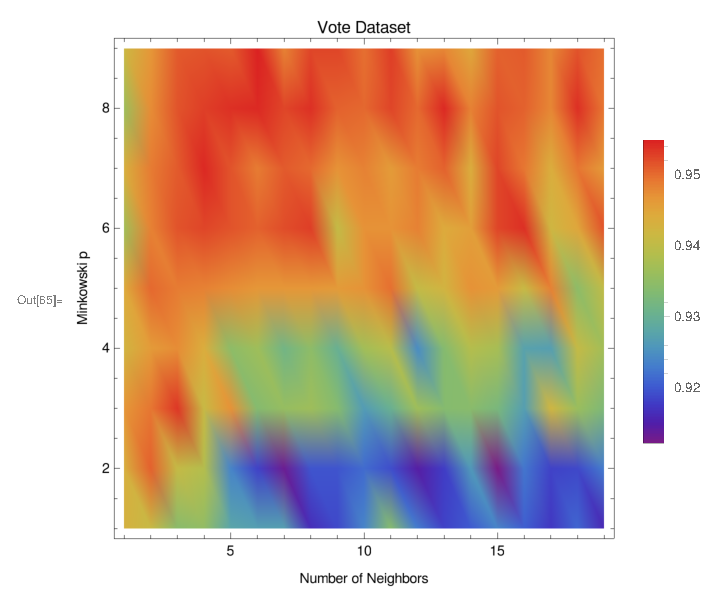
\includegraphics[width=\textwidth]{figs/kNN/vote_plot_kp}	
					\caption{}
					\label{kp_vote}				
				\end{subfigure} \	
				\begin{subfigure}[b]{0.32\textwidth}
					\centering
					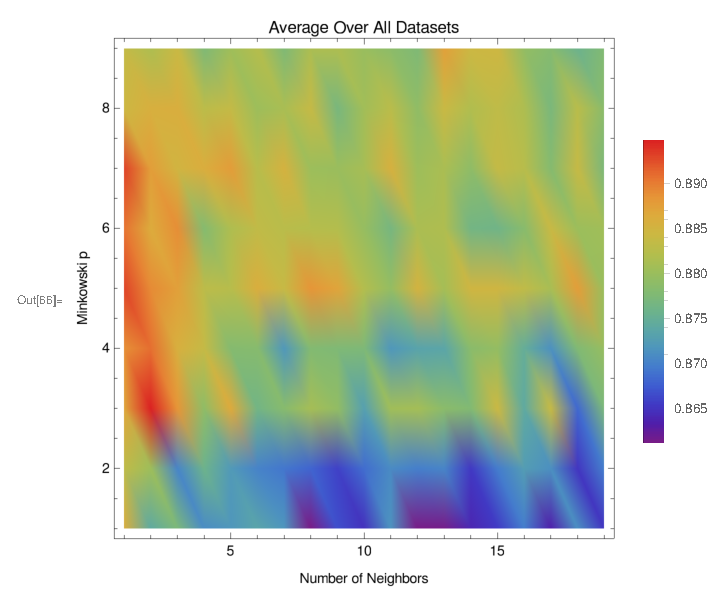
\includegraphics[width=\textwidth]{figs/kNN/average_plot_kp}	
					\caption{}
					\label{kp_ave}				
				\end{subfigure}
				\caption{A series of plots demonstrating the precision (in color) of $k$ nearest-neighbors for different values of $k$ and the $p$ value in the Minkowski distance. We have plotted the response of kNN for all five datasets (Figure \ref{kp_cancer} - \ref{kp_vote}) and the average response over all datasets, Figure \ref{kp_ave}.}
				\label{kp_plot}
			\end{figure}
		
\section{Naive Bayes}
	\label{nbw}

	\textit{Naive Bayes} uses the principle of Bayesian learning to solve the classification problem. 
	This algorithm is said to be naive because it considers the attributes to be conditionally independent when performing classifications. 
	Under this scheme, the probability distribution of each class $C$ is given the set of attributes $x_1,...,x_n$ is written by \cite{ai} as
	\begin{equation}					
		\ve{P}(C|x_1,...,x_n) = \alpha \ve{P}(C) \prod_i \ve{P}(x_i| C)
		\label{nb_pd}
	\end{equation}	
	where, using the maximum likelihood hypothesis, $\ve{P}(C)$ is the prior probability of the class $C$ in the training dataset, $\ve{P}(x_i|C)$ is the likelihood of attribute $x_i$ given $C$, and $\alpha$ is a normalization constant. 
	To find $\ve{P}(C)$ the we simply say it is equal to the proportion of $C$ observed in the training dataset. 
	Similarly, we can calculate the likelihood using the definition of conditional probability
	\begin{equation*}
		P(a|b) = \frac{P(a \land b)}{P(b)}
	\end{equation*}
	where the probabilities are calculated using the number of occurrences in the training dataset. 

	\subsection{Training}
		\label{nb_train}
		
		\begin{figure}[h!]
			\centering
			\begin{subfigure}[b]{0.32\textwidth}
				\centering
				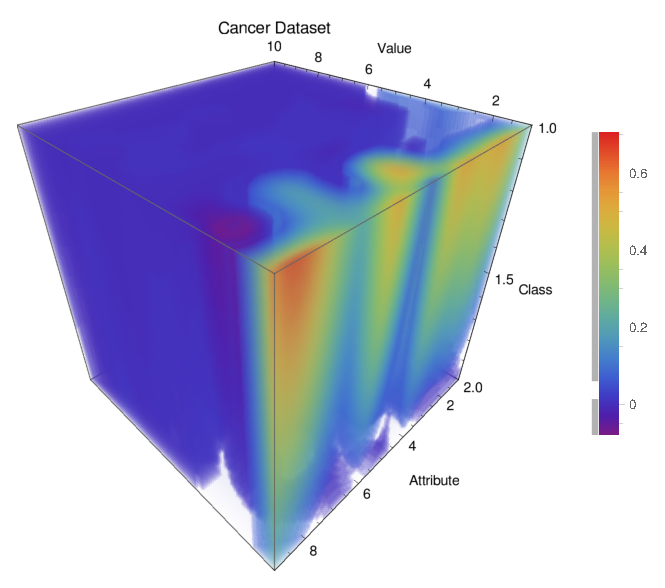
\includegraphics[width=\textwidth]{figs/NaiveBayes/plot_ptable_cancer}	
				\caption{}
				\label{p_cancer}				
			\end{subfigure}	\	
			\begin{subfigure}[b]{0.32\textwidth}
				\centering
				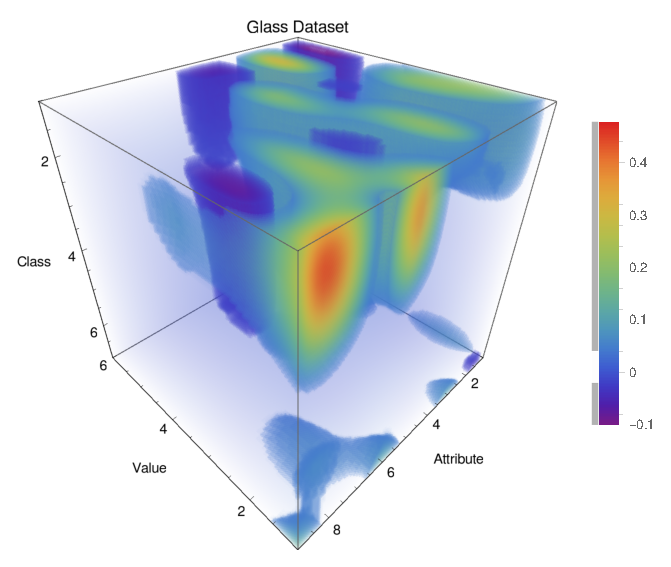
\includegraphics[width=\textwidth]{figs/NaiveBayes/plot_ptable_glass}
				\caption{}
				\label{p_glass}					
			\end{subfigure} \	
			\begin{subfigure}[b]{0.32\textwidth}
				\centering
				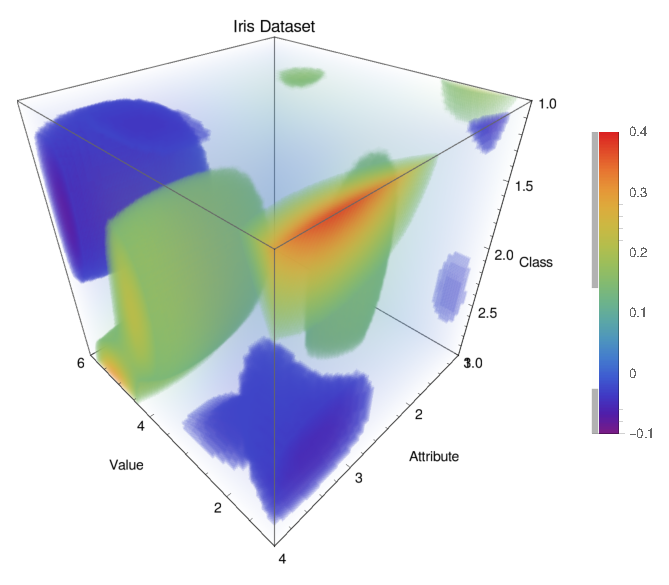
\includegraphics[width=\textwidth]{figs/NaiveBayes/plot_ptable_iris}	
				\caption{}
				\label{p_iris}				
			\end{subfigure} \	
			\begin{subfigure}[b]{0.32\textwidth}
				\centering
				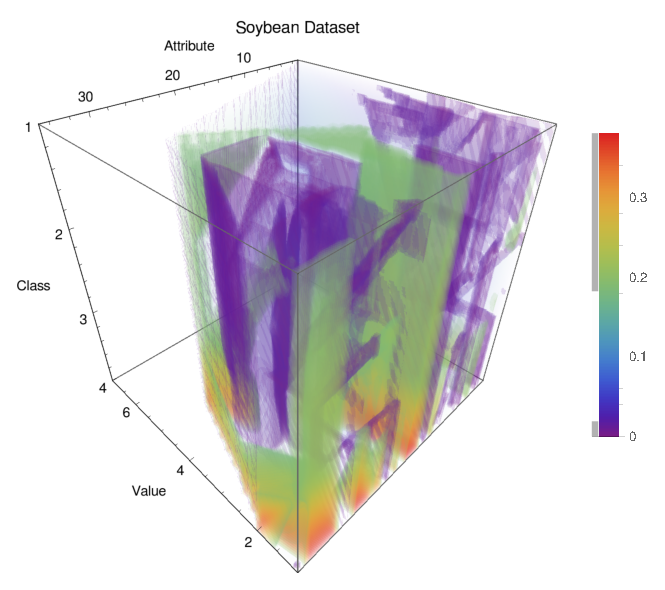
\includegraphics[width=\textwidth]{figs/NaiveBayes/plot_ptable_soybean}	
				\caption{}
				\label{p_soybean}				
			\end{subfigure} \	
			\begin{subfigure}[b]{0.32\textwidth}
				\centering
				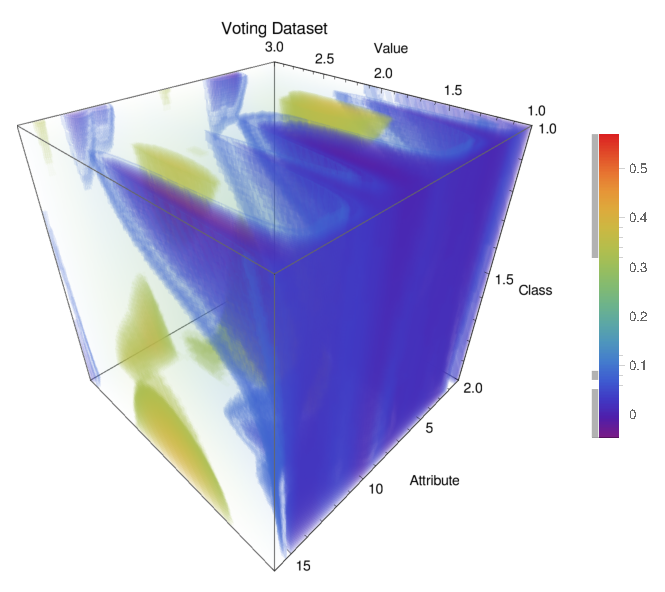
\includegraphics[width=\textwidth]{figs/NaiveBayes/plot_ptable_vote}	
				\caption{}
				\label{p_vote}				
			\end{subfigure}
			\caption{3D density plots of the naive Bayes probability table for all five datasets. The vertical class axis represents the value of the class, $c$, the attribute axis denotes the index of an attribute, $x$, and the value axis represents the vale of that attribute, $a$. Finally the color is equivalent to the probability of the attibute $x$ having value $a$, and the class having the value $c$}
			\label{ptable}
		\end{figure}
			
		During the training phase for naive Bayes, the algorithm simply counts the how many times a specific attribute takes on a particular value for each class. 
		From these counts we build the probability table visualized in Figure \ref{ptable}. 
		In Figure \ref{ptable}, we have plotted the class vs. attribute index vs. attribute value vs. probability (in color) for each of the five datasets. 
		These plots are interesting because they serve to visualize the relationships between classes and attribute values. 
			
		If we contemplate the plots in Figure \ref{ptable}, we can start to visualize how Naive Bayes works. 
		For the cancer dataset in Figure \ref{p_cancer}, we can see how benign (class = 1) results are characterized by low values for every attribute. 
		In the glass dataset, Figure \ref{p_glass}, the low classes (building and vehicle windows) are very well characterized by the attributes, while the miscellaneous glass types (containers, tableware, headlamps) were not dependent upon the attributes. 
		In the iris dataset (Figure \ref{p_iris}), we can see beautiful regions that characterize each species. 
		The soybean dataset in Figure \ref{p_soybean} demonstrates a probability table with an interesting geometric structure, while in the voting dataset, Figure \ref{p_vote}, it seems almost as if we can see the party line between Democrats and Republicans.
				
	\subsection{Validation}
		\label{nbv}
		
		To validate our naive Bayes classifier, we simply use the probability table discussed in Section \ref{nb_train} and Equation \ref{nb_pd} to find the most probable class. 
		To evaluate Equation \ref{nb_pd}, our implementation looped over the classes to construct the product of the conditional probabilities. $P(C)$ was calculated by taking the total occurrences of each class and dividing by the total size of the dataset. $P(x_i | C)$ was found by taking the number of times an attribute $i$ with a specified class $C$ had value $x_i$  divided by the total number occurrences of class $C$;
		
\section{TAN}

		\textit{Tree-Augmented Naive Bayes} (TAN) is an extension to the naive Bayes algorithm described in Section \ref{nbw}. 
		Developed by \cite{Friedman1997}, TAN relaxes the assumption that the attributes are conditionally independent and allows each attribute to depend on only one other attribute. 
		It accomplishes this by constructing a fully-connected, undirected graph out of the attributes in the dataset. 
		TAN then assigns a weight to each connection in the graph using the \textit{conditional mutual information function}, given by	
		\begin{equation*}
			I_P(\ve{X};\ve{Y} | \ve{Z}) = \sum_{\ve{x},\ve{y},\ve{z}} P(\ve{x},\ve{y}, \ve{z}) \log \left( \frac{P(\ve{x},\ve{y} | \ve{z})}{P(\ve{x}|\ve{z})P(\ve{y}|\ve{z})} \right).
			\label{cmi}
		\end{equation*}		
		Applying the this weight to the edges allows us to construct a maximum spanning tree of the graph. 
		We can then make the spanning tree directed by choosing a root node and setting the direction of all edges to be outward from it.
		
		Using this representation, we can calculate the analog of Equation \ref{nb_pd}, the probability distribution, using the expression given by \cite{Zheng2010}
		\begin{equation}
			\text{class} = \text{argmax}_C \left[ P(C) P(x_r | C) \prod_{x_i,x_j} P(x_j | x_i , C) \right]
			\label{tan_pd}
		\end{equation}	
		where $x_i$ is the parent of the attribute $x_j$ in the directed maximum spanning tree and $x_r$ is the root node of the spanning tree.

	\subsection{Training}
		
		To accomplish the TAN algorithm, we will need to construct a probability table similar to the one described in Section \ref{nbw} on naive Bayes. For this algorithm however, the 4D (class, attribute index, attribute value, count) probability table of naive Bayes needs to be extended to a 6D probability table where the dimensions are: class, attribute 1 index, attribute 1 value, attribute 2 index, attribute 2 value, count, to represent probabilites of the form $P(x_i,x_j,C)$, the probability of attributes $i$ and $j$ having the values $x_i$ and $x_j$ and the class value $C$. Unfortuantely, since the dimensionality is so high, constructing plots to visualize the probability table such as Figure \ref{ptable} is impossible.
		
		Once we have iterated through the dataset and constructed our 6D probability table, we can construct a fully connected graph between the attributes using the weight provided by Equation \ref{cmi}. With this fully connected graph, we can use Kruskal's algorithm to construct our maximum spanning tree. This algorithm is best described in the words of Kruskal himself,
		\begin{quote}
			Perform the following step as many times as possible: Among the edges of $G$ not yet chosen, choose the shortest edge which does not form any loops with those edges already chosen. Clearly the set of edges eventually chosen must form a spanning tree of G, and in fact it forms a shortest spanning tree \cite{kruskal}.
		\end{quote}
		To implement Kruskal's algorithm, we started with our fully connected tree weighted by the conditional mutual information functon. Next, we sorted the weights by descending weight, to ensure we end up with a maximum spanning tree. At this point, the fast way to implement this algorithm would be to use a disjoint set data structure, to detect loops while building the MST. We did not use a disjoint set data structure, instead we detected loops by doing a complete depth first search through the tree while testing if each node had already been visited by the DFS. If a node was visited twice, the graph contained a loop. 
		
		\begin{figure}
			\centering
			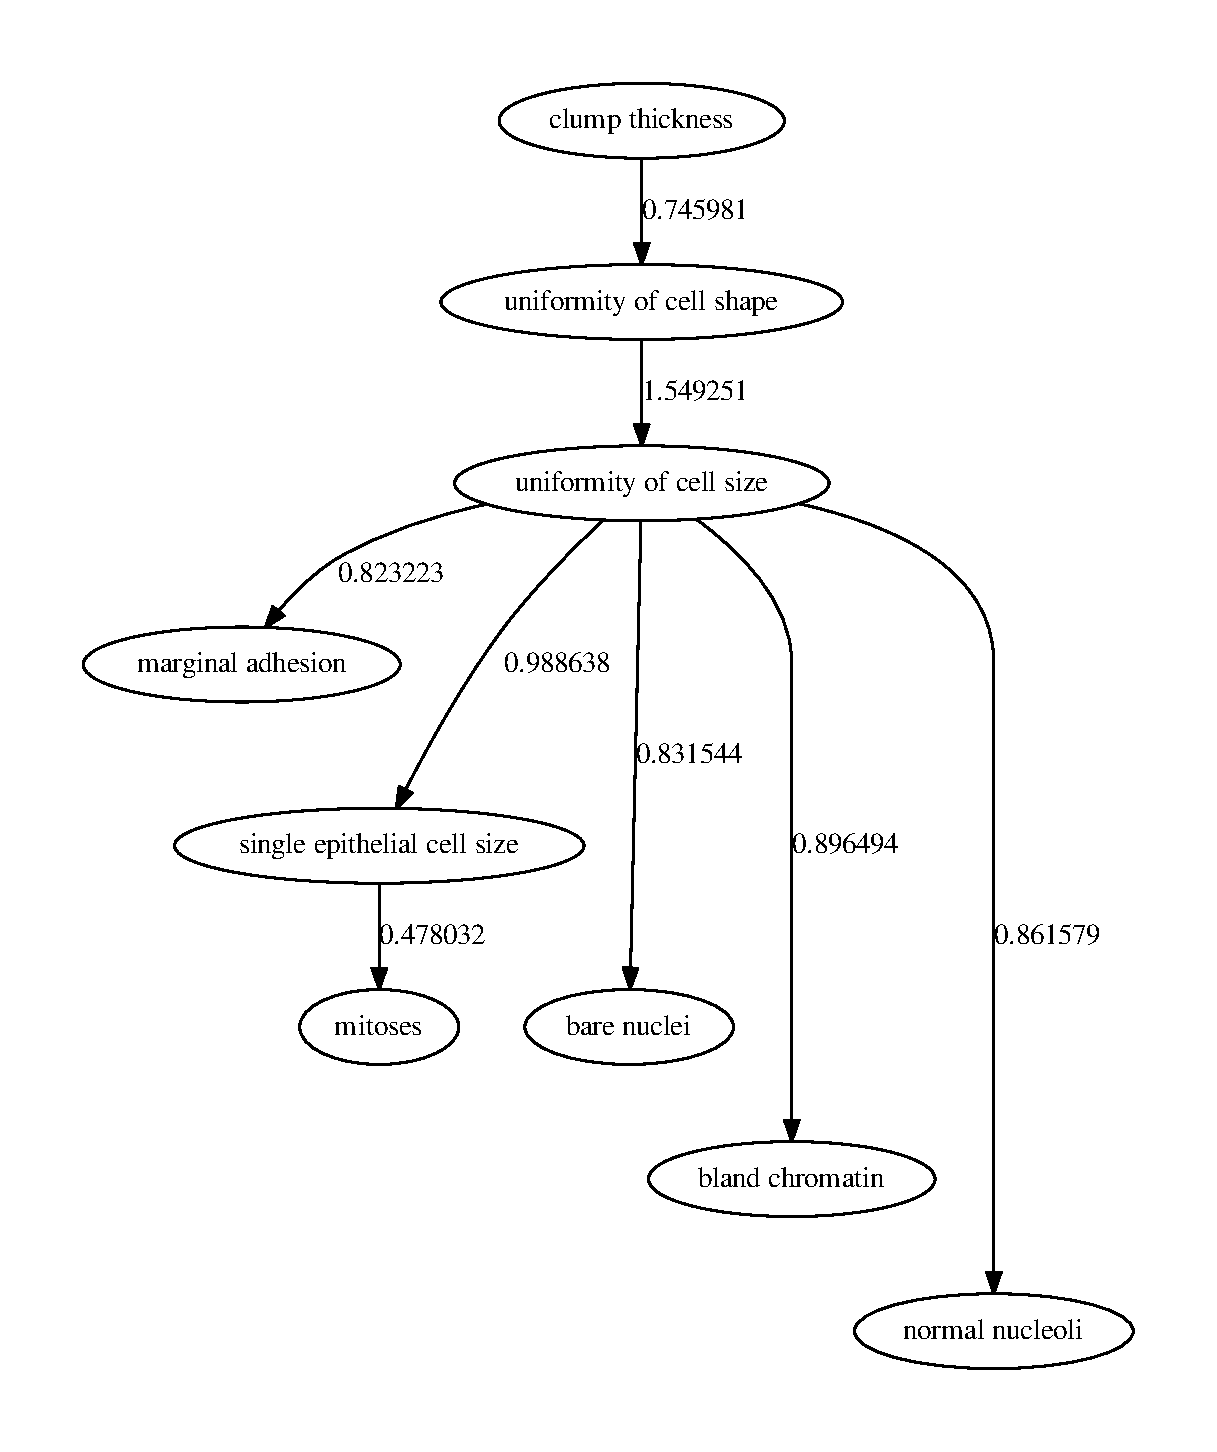
\includegraphics[width=0.5\textwidth]{figs/TAN/cancer}
			\caption{Example of the maximum spanning tree produced by TAN on the cancer dataset.}
		\end{figure}
		
		Using our loop detection function, we were able to build MSTs describing the ``largest'' dependence of one attribute on another. With the MST complete, TAN is ready for validation.
		
	\subsection{Validation}
		
		The validation phase of TAN is similar to the validation of naive Bayes described in Section \ref{nbv}. The only difference is that we use the MST built in preceding section to determine the parent of each node. We then used Equation \ref{tan_pd} and our 6D probability table to determine the most probable class.
		
\section{ID3}
	\subsection{Training}
	\subsubsection{Tree Construction}
	The \texttt{id3} method was the main logic behind tree construction. We closely followed the decision tree learning psuedocode in Figure 18.5 in \cite{ai}. 
	ID3 is an recursive process that generates a short tree by splitting the tree one attribute at a time. 
	The first attribute to be used is the one with the most information gain. 
	Information gain can described as how much entropy the system lost by splitting on an attribute. 
	The equation for entropy is as follows:
	\begin{equation*}
		H(S) = \sum_{i=1}^{n} \left( -p_i \log_2 p_i \right). 
	\end{equation*}		
	where $p_i$ is the proportion of the number of datums in class $i$ to the total number of datums in the set $S$. 
	To use this equation the entropy of the whole system is determined first. 
	Then the sum of the entropy for each new branch is calculated and subtracted from the total entropy. We try to branch on each attribute that has not been used yet. Since the goal is to maximize this difference so the tree will be small and more general, we choose the attribute that resulted in the greatest reduction of entropy. The reduction of entropy is defined as information gain.
	The rest of the algorithm is just iterating through the tree as it is made and recursively performing the calculation on an attribute that has not been split yet. 
	The tree is finished when all leaf nodes are a single class or when attributes to split on have run out.
	In this case each leaf node that does not have a class is assigned the most common class in that leaf.
	
	Do deal with continuous variables we just used the discretization method outlined above.
	
	\begin{figure}[h]
		\centering
		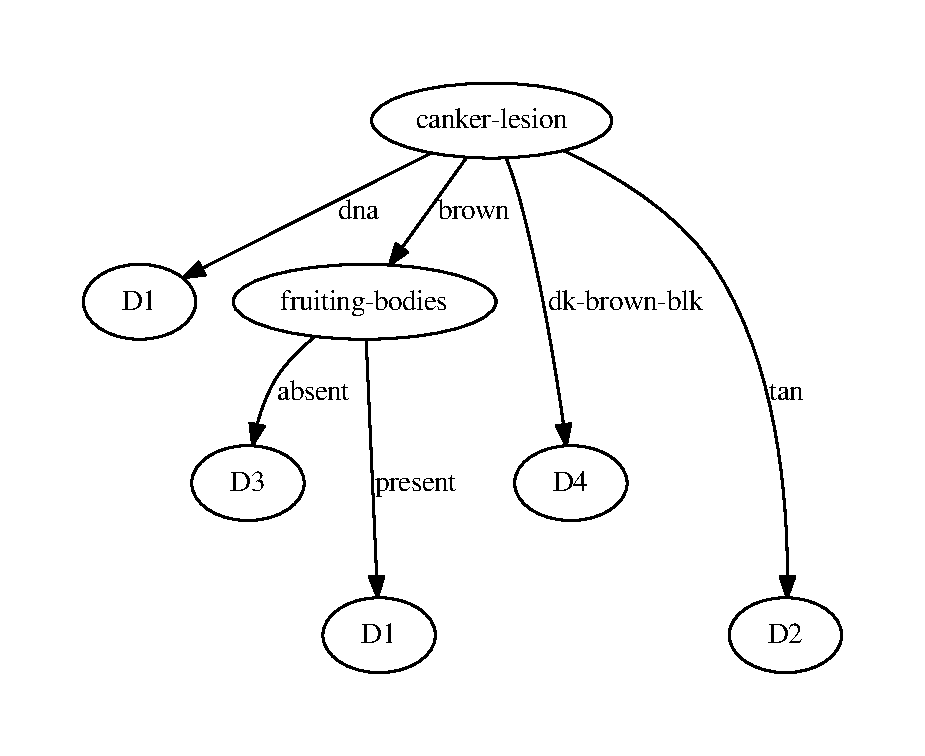
\includegraphics[width=0.5\textwidth]{figs/ID3/soybean}
		\caption{An example id3 tree generated for the soybean database.}
		\label{tan}
	\end{figure}
	\subsubsection{Pruning}
	We implemented reduced error pruning to help make the tree more general. The approach was to split the training set into a smaller training set and a validation set. The tree was then generated as usual using the new training set. We then removed non-leaf nodes one at a time, checking how well they performed on the validation set. If they performed better, the nodes remained removed. Otherwise they would be restored to their previous state.
	\subsection{Validation}
	The process of classifying a datum according to the tree is a simple process. The tree is traversed according to the values of each variable in the datum. When a leaf node is reached, that leaf's class is returned. It is easy to determine leaf nodes because they lack children nodes.
	
\section{Results}
	To show the relationship between training set size and precision we created the graphs seen in Figure  \ref{conv_plot}.

	
		\label{conv}
		\begin{figure}[h!]
			\centering
			\begin{subfigure}[b]{0.49\textwidth}
				\centering
				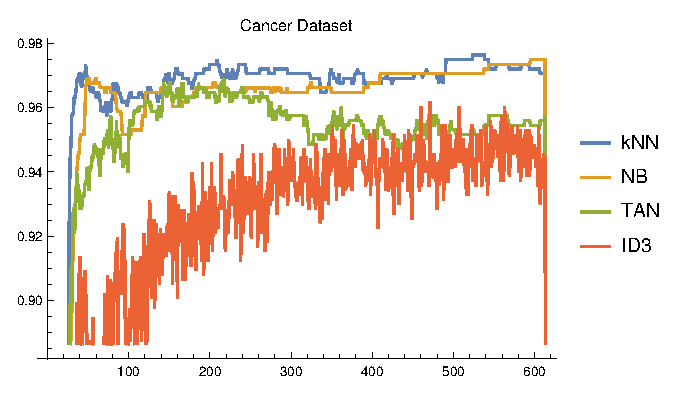
\includegraphics[width=\textwidth]{figs/plot_conv_cancer}		
				\caption{}	
				\label{conv_cancer}		
			\end{subfigure}	\	
			\begin{subfigure}[b]{0.49\textwidth}
				\centering
				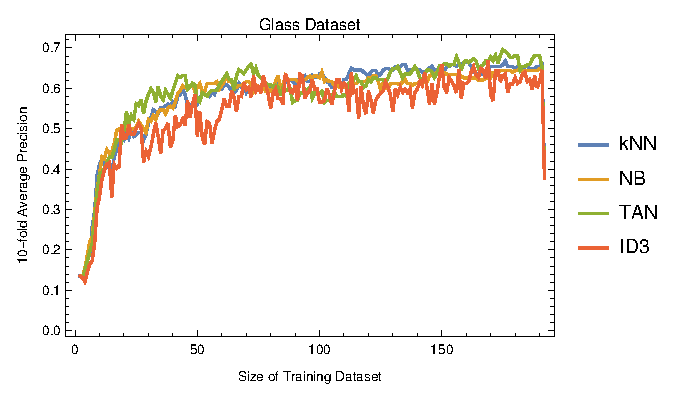
\includegraphics[width=\textwidth]{figs/plot_conv_glass}
				\caption{}
				\label{conv_glass}					
			\end{subfigure} \	
			\begin{subfigure}[b]{0.49\textwidth}
				\centering
				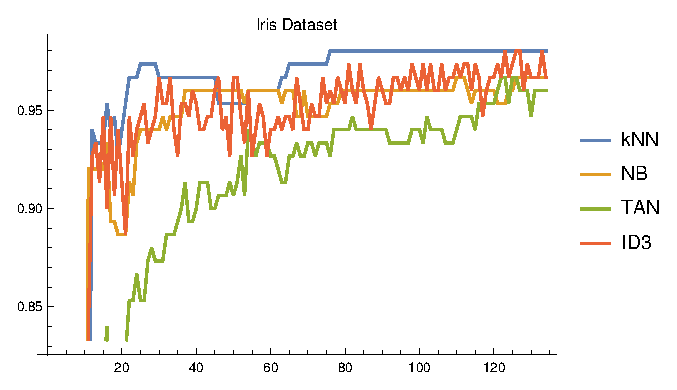
\includegraphics[width=\textwidth]{figs/plot_conv_iris}	
				\caption{}		
				\label{conv_iris}			
			\end{subfigure} \	
			\begin{subfigure}[b]{0.49\textwidth}
				\centering
				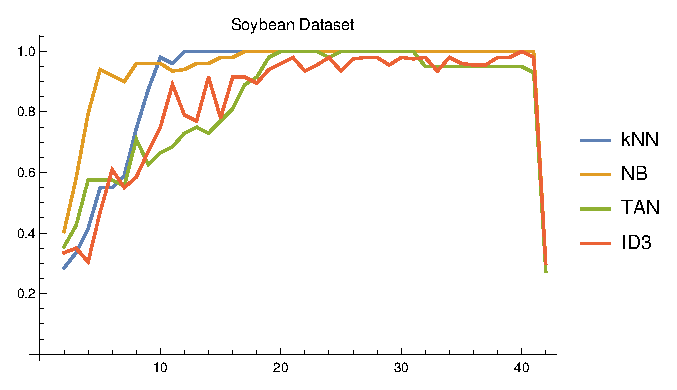
\includegraphics[width=\textwidth]{figs//plot_conv_soybean}		
				\caption{}
				\label{conv_soybean}				
			\end{subfigure} \	
			\begin{subfigure}[b]{0.49\textwidth}
				\centering
				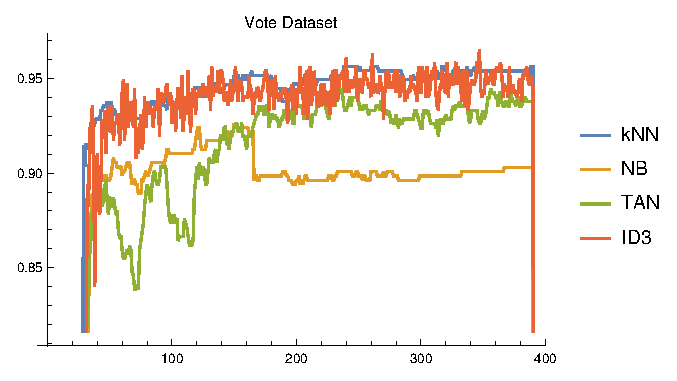
\includegraphics[width=\textwidth]{figs/plot_conv_vote}			
				\caption{}	
				\label{conv_vote}		
			\end{subfigure}
			\caption{Plot showing the learning curves for each of the algorithms on the five datasets. Please note the low point on the right hand side of Figures \ref{conv_cancer}, \ref{conv_glass},  \ref{conv_soybean},\ref{conv_vote} is in error and is not part of our results.}
			\label{conv_plot}
		\end{figure}
		
		\begin{table}[h!] 
			\centering
			
			\begin{tabular}  { | l | l | l | l | l | l | l | }
				\hline
			\rowcolor{gray}	& \textbf{Cancer} & \textbf{Glass} & \textbf{Iris} & \textbf{Soybean} & \textbf{Vote} & Average \\
				\hline
				\cellcolor{gray} \textbf{kNN} & 0.953154  & \cellcolor{red}0.579221 & 0.96 & \cellcolor{green}1 & 0.942389 & \cellcolor{red}0.8869528  \\
				\hline
			\cellcolor{gray}	\textbf{NB} & \cellcolor{green}0.975085 & 0.649783 &\cellcolor{red} 0.95333 & \cellcolor{green}1 & \cellcolor{red}0.903436 & \cellcolor{lightgray}0.8963268   \\
				\hline
			\cellcolor{gray}	\textbf{TAN} & 0.961893 & \cellcolor{green}0.66342 & 0.96 & 0.98 & 0.944767 & \cellcolor{lightgray}0.902016 \\
				\hline
			\cellcolor{gray}	\textbf{ID3} & \cellcolor{red}0.950171 & 0.662771 & \cellcolor{green}0.98 & \cellcolor{red}0.975 & \cellcolor{green}0.95629 & \cellcolor{green}0.9048464 \\
				\hline
			\rowcolor{lightgray}	\cellcolor{gray} Average & 0.960 & 0.639 & 0.9633325 & 0.98875 & 0.9367205 & \\
				\hline
				
			\end{tabular}
			\caption{1x10 Cross Validation Precision. Green represents the best performing algorithm for each data set. Red represents the worst.}
			\label{table}
		\end{table}
		
		\subsection{Cancer Dataset Performance}
		
			In the cancer dataset, $k$NN and naive Bayes obtained very similar results in terms of precision. We can see that $k$NN had the fastest learning curve, staying dominant until the training set was larger than 400 items where naive Bayes finally caught up. The results from TAN were mildly suprising since the algorithm had a maximum in accuracy at a training set size of 150. ID3 poorly on this dataset compared to other algorithms, displaying a slow training time and precision lower than that of TAN.
		
		\subsection{Glass Dataset Performance}
		
			The glass dataset was easily the most difficult of the five datasets for all algorithms. However, TAN did really well on this dataset, displaying the fastest learning curve and nearly tied for the best in final precision with a value of 66\%. $k$NN and naive Bayes did similarly, to the other two algorithms (which was still not great).
		
		\subsection{Iris Dataset Performance}
		
			The iris dataset was a fairly easy dataset for most of our MLAs to solve. $k$NN did the best, consistenty getting perfect classifications with training sets larger than 80 members. Naive Bayes and ID3 had approximately the same performance on this dataset, displaying a similar learning curve to $k$NN, but failing to keep up compared to $k$NN as the training sets increased in size. TAN did exceptionally poorly on this dataset, in having a much slower learning curve than the other three algorithms.
		
		\subsection{Soybean Dataset Performance}
		
			As previously mentioned, the soybean dataset was the smallest out of the five datasets. Therefore the validation dataset was very small for 10-fold cross-validation, which may have made our algorithms appear more precise than reality. Nonetheless $k$NN and naive Bayes did the best on this dataset, having the fastest learning curves and perfect accuracy on the full training dataset. ID3 and TAN appear to have slower learning curves, but the accuracy of these algorithms was still very high on the full dataset.
		
		\subsection{Voting Dataset Performance}
		
			The voting dataset was the best performance for the ID3 algorithm, although $k$NN still displayed very similar performance. Most surprising about this dataset is the performance of naive Bayes, which started off with a similar learning curve to ID3 and $k$NN, but settled at a local maximum at a training dataset size of approximately 130 members before taking a sharp dive in precision at about 160 members in the training set. TAN showed an almost opposite precision response, with poor accuracy between 50 and 120 training dataset members and better with increasing training set size.

\section{Conclusion}
	

	\pagebreak


	%\bibliographystyle{apj}
	\bibliographystyle{apalike}
	
	\bibliography{sources}
\end{document}
